\documentclass[14pt]{matmex-diploma}
\usepackage{tikz}
\usepackage{pgfplots}
\pgfplotsset{compat=1.9}

\begin{document}
\filltitle{ru}{
    chair              = {Кафедра Системного программирования},
    title              = {Синтаксический анализ графов с помеченными вершинами и ребрами},
    type               = {coursework},
    position           = {студента},
    group              = 344,
    author             = {Ершов Кирилл Максимович},
    supervisorPosition = {ст. преп., к.\,ф.-м.\,н.},
    supervisor         = {Григорьев С.\,В.},
}
\maketitle
\tableofcontents
\section*{Введение}

\section{Постановка задачи}
\begin{itemize}
    \item В рамках проекта YaccConstructor \cite{YaccConstructorPage} реализовать возможность поиска путей в графе с помеченными вершинами и рёбрами по заданной КС-грамматике.
    \item Реализовать удобный интерфейс для работы:
    \begin{itemize}
    \item создание и выполнение запросов 
    \item получение и обработка результатов
    \end{itemize}
    \item Провести апробацию и сравнить с существующими решениями.
    
\end{itemize}

\section{Обзор}

\subsection{Синтаксический анализ графов}

\subsection{YaccConstructor и QuickGraph.Query}

\section{Реализация}
В YaccConstructor есть абстрактная реализация алгоритма синтаксического анализа GLL. Исходная грамматика описывается на языке спецификации грамматик YARD. Затем генератором из неё извлекается необходимая для работы алгоритма информация о грамматике. Во время выполнения алгоритм перемещается по входному объекту в зависимости от текущей позиции в грамматике. Объект, в котором требуется найти пути, удовлетворяющие исходной КС-грамматике, должен реализовывать интерфейс IParserInput. В рамках данной работы был реализован этот интерфейс для графов с помеченными вершинами и рёбрами. Если текущая позиция --- вершина, следующими позициями в графе являются все исходящие рёбра. Если текущая позиция на ребре, следующей является конечная вершина. Таким образом, алгоритмом проверяются все возможные пути в графе. Результатом работы программы является sppf (лес разбора). Также для графа можно задать вершины, с которых будет начинать работу алгоритм и вершины, являющиеся конечными для синтаксического анализа. Для проверки работы алгоритма были написаны тесты.

В проекте QuickGraph.Query есть метод, извлекающий подграф из sppf. Но возвращает он граф с метками только рёбрах. Дополнительно была реализована возможность извлечения подграфа с метками на вершинах и рёбрах. Также реализована печать графа с метками на вершинах в dot-файл. Этот формат удобен для графического представления графов.

\section{Эксперименты}
\subsection{Данные}

\begin{figure}
\centering
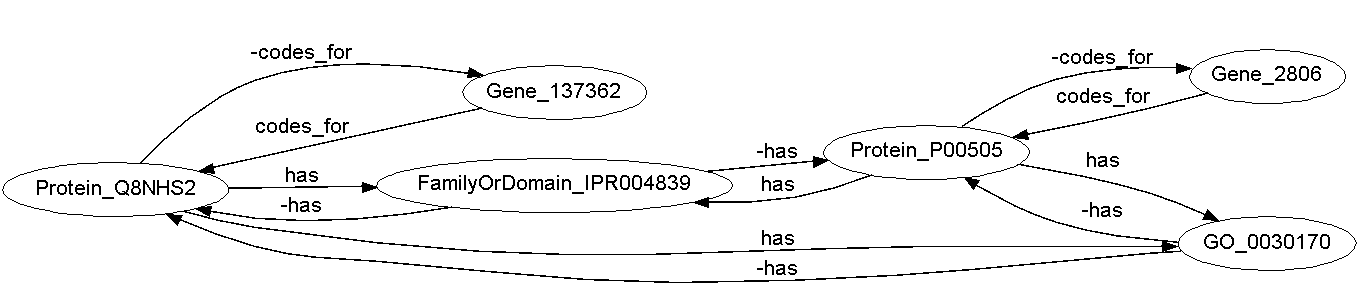
\includegraphics[width=16cm]{images/subgraph1.png}
\caption{Пример подграфа}
\label{subgraph}
\end{figure}

Существует большое количество биологических баз данных с открытым доступом, информация в которых может быть представлена как помеченный граф, в котором вершины соответствуют сущностям (протеины, гены, фенотипы), а рёбра отношениям между ними (взаимодействует, кодирует). Пути между вершинами позволяют найти новые связи в данных, либо показывают уже известные отношения. Подграф, построенный на всех найденных путях, более наглядно демонстрирует связи между вершинами. На рисунке \ref{subgraph} показан пример подграфа, построенного на путях между генами. 

Реальный набор биологических данных был собран из разных баз данных, находящихся в открытом доступе:  Entrez Gene (информация о генах), UniProt (протеины), Gene Ontology (биологические процессы), STRING (связи между протеинами), InterPro (семейства белков), KEGG (связи между генами), HomoloGene (группы гомологий генов). Данные были ограничены набором из пяти организмов: Homo sapiens, Rattus norvegicus, Mus musculus, D. melanogaster и C. elegans. Объединенные в один файл данные состоят из троек: субъект, отношение, объект. Такие тройки образуют помеченный ориентированный граф.
\subsection{Запросы}

\begin{figure}
$$
\begin{array}{crcl}
&\mbox{\texttt{ [<Start>] }} \\
&\mbox{\texttt{s}} &:& \mbox{\texttt{gene }} \\
&\mbox{\texttt{v}} &:& \mbox{\texttt{protein | gene | GO | PATHWAY | FAMDOM | HOMOLOGENE}} \\
&\mbox{\texttt{similar}} &:& \mbox{\texttt{CODESFOR v RCODESFOR | BELONGS v RBELONGS}} \\
&&&\mbox{\texttt{| HAS v RHAS | HOMOLOGTO v RHOMOLOGTO}} \\
&\mbox{\texttt{ps}} & :& \mbox{\texttt{ (PROTEIN similar) *[1..2]}} \\
&\mbox{\texttt{protein}} & :& \mbox{\texttt{ps PROTEIN | PROTEIN}} \\
&\mbox{\texttt{gs}} & :& \mbox{\texttt{(GENE similar) *[1..2]}} \\
&\mbox{\texttt{gene}} & :& \mbox{\texttt{gs GENE | GENE}} \\
\end{array}
$$
\caption{Грамматика на языке YARD}
\label{grammar}
\end{figure}

Все вершины в полученном графе имеют уникальную метку. Но для удобства будем различать их по типу: гены, фенотипы и т.д. Назовём две вершины в графе похожими, если они одного типа и имеют рёбра одного типа к похожим вершинам. Это определение рекурсивно. Таким образом, путь между похожими вершинами представляет собой палиндром, который нельзя задать с помощью регулярной грамматики. На рисунке \ref{grammar} показана КС-грамматика на языке YARD, которая определяет похожие гены.  
\subsection{Производительность}

\begin{figure}
\begin{center}
\begin{tikzpicture}
\begin{axis}[
    xlabel = {Количество рёбер, тыс},
    ylabel = {Время, с}
]
\addplot coordinates {
  (1.048,0.2) (2.334,0.68) (4.742,3.2) (7.046,8.7) (9.850,17.5) (12.398,30.7) (14.968,51.3) (17.432,84.2) (20.480,132)
};
\end{axis}
\end{tikzpicture}
\end{center}
\caption{Время работы алгоритма}
\label{time}
\end{figure}

Для оценки производительности была проведена серия экспериментов. Результаты приведены на графике, изображённом на рисунке \ref{time}. В статье \cite{subgraph} был проведён похожий эксперимент, но длины путей были ограничены от 4 до 8. В данной работе добиться такого ограничения не удалось, подграф строится по путям любой длины, поэтому нет возможности напрямую сравнить результаты.

\section{Заключение}

\setmonofont[Mapping=tex-text]{CMU Typewriter Text}
\bibliographystyle{ugost2008ls}
\bibliography{diploma.bib}
\end{document}
